\chapter{Arquitectura y tecnologías}
\label{chapter:arquitectura}

El objetivo de este capítulo es tener un diseño esquemático de la solución planteada, este diseño será abordado en primer lugar desde un punto de vista lógico, de acuerdo a las necesidades del proyecto, posteriormente aterrizaremos esta arquitectura con tecnologías concretas que nos ayuden a conseguir el objetivo deseado.

\section{Arquitectura}
\begin{figure}[!ht]
	\centering
	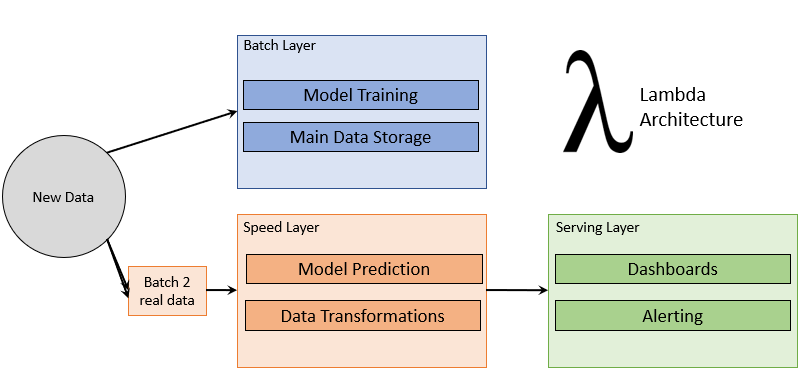
\includegraphics[width=1\textwidth]{images/arqu/lambda}
	\caption{Arquitectura Lambda propuesta}
	\label{fig:lambda}
\end{figure}




En este apartado definiremos la arquitectura desde un punto de vista lógico, esta arquitectura debe responder a los objetivos propuestos para cumplir con las necesidades de negocio existentes. 


En líneas generales, podemos ver la arquitectura de nuestro sistema como una arquitectura \textit{Lambda} en la que disponemos de una capa \textit{batch}, una capa rápida o \textit{real-time} y una última capa de servicio.



La capa batch será la encargada de entrenar el modelo a través de los datos de las llamadas, la capa rápida obtendrá los \textit{topics} de las llamadas en tiempo real usando el modelo previamente entrenado y por último la capa de servicio será la encargada de mostrar estos datos al usuario mediante cuadros de mando.  

En la Figura \ref{fig:lambda} podemos ver un esquema general de nuestra arquitectura. A continuación definimos con más detalle cada una de las capas del modelo.




\subsection{Capa Batch}
El \textit{core} del proyecto que abordamos es el modelo, encargado de extraer los \textit{topics} de las transcripciones de llamadas al servicio de atención al cliente. Este modelo debe entrenarse usando un histórico suficientemente amplio. 

El modelo es un elemento vivo en nuestra arquitectura y, además de por posibles mejoras en los hiperparámetros o por la tecnología, debe re-entrenarse conforme se vayan recibiendo datos nuevos en el histórico, ya que es lógico pensar que la temática de las consultas variarán a lo largo del tiempo debido por ejemplo al lanzamiento de nuevos productos. 


\subsection{Capa Real-Time}
La \textit{speed layer} de nuestro proyecto será la encargada de recibir los datos en tiempo real, las llamadas serán publicadas en un bus de eventos y estos eventos serán consumidos por una capa de procesamiento que será la encargada de aplicar el modelo entrenado en la capa \textit{batch} a los nuevos datos. Los \textit{topics} resultantes de cada llamada serán publicados de nuevo en este bus para poder ser ingestados posteriormente a una BBDD NO-SQL, que será la encargada de proporcionar la información a la capa de servicio. 

Aprovecharemos también las características de la BBDD NoSQL para, mediante un módulo de \textit{Machine Learning}, detectar anomalías en series temporales y poder alarmar en el caso de que un \textit{topic} concreto se dispare en algún momento.  

Debido a la situación actual, las llamadas no se ingestan en \textit{real-time} si no que se procesan en mini \textit{batches} cada cierto tiempo. Es muy probable que este escenario cambie en el futuro por lo que se construirá un elemento de entrada a la capa rápida que transformará el mini-batch en eventos conforme vayan ejecutándose (este elemento puede observarse en la figura \ref{fig:lambda} como \textit{Batch 2 real data}). Esta pieza será suprimida una vez las llamadas sean recibidas en tiempo real. 


\subsection{Capa de Servicio}
Una vez almacenados los datos en la BBDD debemos construir un frontal que muestre al usuario el número de llamadas analizadas, el modelo utilizado y principalmente la evolución de los \textit{topics} a lo largo del tiempo. 

Lo ideal es que esta capa de servicio se vaya actualizando en tiempo cuasi-real y permita a los diferentes usuarios realizar cuadros de mando personalizados según sus necesidades. 

Otro requisito esencial en este tipo de proyectos es que la información este disponible vía API-REST para poder ser consumida por terceros.    


\section{Integración y Despliegue Continuos}
Como ya hemos visto al hablar del entrenamiento del modelo, el desarrollo de este tipo de proyectos no tiene un principio y un final, si no que se trata de un proceso cíclico en el que por necesidades del negocio, por cambio en los datos o por cambio en la tecnologías, será necesario añadir mejoras o modificaciones en nuestro desarrollo. 

Por estos motivos es conveniente definir mecanismos que nos permitan, tras cada cambio efectuado, poder realizar las pruebas necesarias y desplegar estos cambios de una manera totalmente automatizada y sin intervención del usuario. 

Aunque este apartado queda fuera de la implementación inicial del proyecto es imprescindible llevarlo a cabo para que este sea sostenible a lo largo del tiempo. 


TODO (Posible ampliar con apuntes sobre el ciclo de vida de los datos y contar beneficios de un despliegue continuo)

\section{Tecnologías}

Al igual que la arquitectura descrita anteriormente era la encargada de responder a las necesidades de negocio, las tecnologías descritas en este apartado nos darán las piezas necesarias para poder construir esa arquitectura y dar respuesta a nuestro caso de uso. 


En el proceso de selección de las tecnologías, no solo se ha tenido en cuenta la idoneidad de las mismas para el caso de uso, si no que se ha valorado también la experiencia en la misma y la disponibilidad dentro del entorno de trabajo. Esto puede provocar que en algunos casos aunque la tecnología se adapte al caso de uso, puedan existir otras soluciones más óptimas cuyo uso era menos viable dado los plazos de ejecución del proyecto. 

A continuación enumeraremos las tecnologías agrupadas en las diferentes capas que hemos comentado en el apartado de arquitectura, además añadiremos las tecnologías que se usarán para la integración y despliegue continuo. 

\subsection{Capa batch}

\begin{itemize}
	\item \textbf{Spark}: Es un framework de computación en clúster. Este \textit{framework} se encuentra desplegado sobre un clúster Hadoop, específicamente una distribución HortonWorks, y posee librerías específicas para Machine Learning como MLLIB.
	\item \textbf{Tensorflow} sobre GPUs: Para el entrenamiento de los modelos también disponemos de un cluster con GPUs sobre el que podremos correr código usando la librería de Google Tensorflow para entrenar nuestros modelos.
\end{itemize}

\subsection{Capa Real-Time}

\begin{itemize}
	\item \textbf{Kafka}: Es el \textit{core} de la capa rápida, se trata de un bus de evento distribuido a través del cual se realizara la ingesta o publicación de los eventos (llamadas). Las diferentes capas de procesamiento que requieran estos eventos se suscribirán a este Bus.
	\item \textbf{Microservicios}: En nuestra capa Real Time construiremos diferentes microservicios en la capa de procesamiento, estos microservicios serán por ejemplo los encargados de devolver los \textit{topics} de cada llamada a partir de una llamada API REST. Estos microservicios correran sobre contenedores en una plataforma Openshift. 
	\item\textbf{ Kafka Stream y KSQL}: A la hora de procesar la información en eventos ingestada en nuestro Bus Kafka disponemos de dos herramientas muy potentes que son Kafka Stream y KSQL. El primero consiste en una serie de librerías que nos permiten construir aplicaciones y microservicios cuyo origen y destino sean un Bus Kafka. KSQL en cambio es un motor SQL aplicable a eventos que nos llegan mediante \textit{streaming}.
	\item \textbf{Logstash}: Una vez hayamos extraído los \textit{topics} correspondientes a cada llamada o evento, tendremos que ingestar esta información en nuestra BBDD, que en este caso será Elasticsearch. Logstash nos permitirá leer de Kafka, realizar las transformaciones necesarias y volcar la información resultante en Elasticsearch.
	\item \textbf{Elasticsearch}: Aunque no se trata en el sentido más estricto de una BBDD No-SQL, si no de un motor de búsqueda, Elasticsearch nos permite almacenar la información en forma de documentos json y realizar consultas y agregaciones sobre cualquier campo. Entre las características que podemos aprovechar de Elasticsearch para nuestro objetivo están: 
	\begin{itemize}
		\item Ingesta en tiempo casi real.
		\item Consulta en tiempo casi real. 
		\item Disponibilidad de mecanismos de ingesta (Logstash) y consulta (kibana).
		\item Posibilidad de crear alarmas en base a consultas. 
		\item Posibilidad de crear \textit{jobs} de Machine Learning que detecten anomalías en series temporales. 
	\end{itemize}
	
	
\end{itemize}

\subsection{Capa Servicio}
\begin{itemize}
	\item \textbf{Elasticsearch API REST}: Toda la información almacenada previamente en Elasticsearch puede ser accedida a través de su API REST por lo que será nuestro método de publicación de la información. 
	\item \textbf{Kibana}: Será el frontal donde los usuarios podrán consultar sus diferentes cuadros de mando y construir nuevos de acuerdo a sus necesidades. También, gracias al modulo de \textit{machine learning} de Elasticsearch, los usuarios podrán crear \textit{jobs} de \textit{machine learning} para detectar anomalías en los temas tratados y generar las alertas necesarias.
\end{itemize}


\subsection{Integración y Despliegue Continuo}
Aunque la implementación de esta parte se escapa de los plazos del proyecto, las tecnologías que se usarán para llevarla a cabo serán. 
\begin{itemize}
	\item \textbf{BitBucket}: Será el repositorio usado para almacenar las nuevas versiones de nuestro \textit{software} de manera que podamos tener un control de versiones.
	\item \textbf{Jenkins}: Es un servidor de integración continua \textit{open source}  que mediante la creación de tareas nos ayudará a realizar el \textit{build} de nuestro software realizando de manera automática las pruebas necesarias.
\end{itemize}